\documentclass[11pt]{article}
\usepackage[paperwidth=180in,paperheight=180in]{geometry}
\batchmode
\usepackage[utf8]{inputenc}
\usepackage{amsmath}
\usepackage{amssymb}
\usepackage{stmaryrd}
\newcommand{\R}{\mathbb{R}}

\usepackage[verbose]{newunicodechar}

\newunicodechar{¬}{\ensuremath{\neg}}
\newunicodechar{Γ}{\ensuremath{\Gamma}}
\newunicodechar{γ}{\ensuremath{\gamma}}
\newunicodechar{λ}{\ensuremath{\lambda}}
\newunicodechar{φ}{\ensuremath{\varphi}}
\newunicodechar{ψ}{\ensuremath{\psi}}
\newunicodechar{ϕ}{\ensuremath{\varphi}}
\newunicodechar{ᵢ}{\ensuremath{{}_{i}}}
\newunicodechar{₀}{\ensuremath{{}_{0}}}
\newunicodechar{₁}{\ensuremath{{}_{1}}}
\newunicodechar{₂}{\ensuremath{{}_{2}}}
\newunicodechar{₃}{\ensuremath{{}_{3}}}
\newunicodechar{₄}{\ensuremath{{}_{4}}}
\newunicodechar{₅}{\ensuremath{{}_{5}}}
\newunicodechar{₆}{\ensuremath{{}_{6}}}
\newunicodechar{₇}{\ensuremath{{}_{7}}}
\newunicodechar{₈}{\ensuremath{{}_{8}}}
\newunicodechar{₉}{\ensuremath{{}_{9}}}
\newunicodechar{ₙ}{\ensuremath{{}_{n}}}
\newunicodechar{ⱼ}{\ensuremath{{}_{j}}}
\newunicodechar{ℓ}{\ensuremath{\ell}}
\newunicodechar{→}{\ensuremath{\rightarrow}}
\newunicodechar{⇒}{\ensuremath{\supset}}
\newunicodechar{⇔}{\ensuremath{\Leftrightarrow}}
\newunicodechar{∅}{\ensuremath{\emptyset}}
\newunicodechar{∈}{\ensuremath{\in}}
\newunicodechar{∘}{\ensuremath{\circ}}
\newunicodechar{∙}{\ensuremath{\bullet}}
\newunicodechar{∧}{\ensuremath{\wedge}}
\newunicodechar{∨}{\ensuremath{\vee}}
\newunicodechar{∼}{\ensuremath{\sim}}
\newunicodechar{≠}{\ensuremath{\neq}}
\newunicodechar{≡}{\ensuremath{\equiv}}
\newunicodechar{⊃}{\ensuremath{\supset}}
\newunicodechar{⊕}{\ensuremath{\oplus}}
\newunicodechar{⊖}{\ensuremath{\ominus}}
\newunicodechar{⊢}{\ensuremath{\vdash}}
\newunicodechar{⊤}{\ensuremath{\top}}
\newunicodechar{⊥}{\ensuremath{\bot}}
\newunicodechar{⊻}{\ensuremath{\veebar}}
\newunicodechar{⟝}{\ensuremath{\vdash}}
\newunicodechar{⬓}{\ensuremath{\square}}
\newunicodechar{Σ}{\ensuremath{\sum}}
\newunicodechar{Π}{\ensuremath{\prod}}

\usepackage{tikz}
\pagestyle{empty}

\setlength{\topskip}{0pt}
\setlength{\parindent}{0pt}
\setlength{\abovedisplayskip}{0pt}
\setlength{\belowdisplayskip}{0pt}

\begin{document}

\begin{minipage}{0.1in}
    \strut\special{dvisvgm:bbox new formula}\special{dvisvgm:raw<!--start {?x} {?y} -->}
\usetikzlibrary{decorations.pathmorphing}
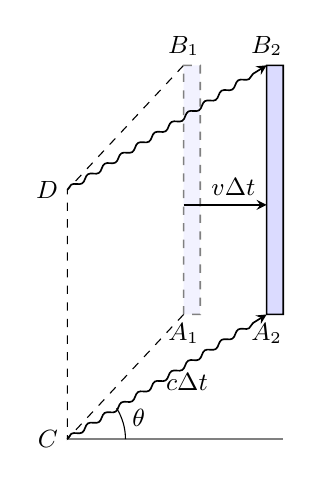
\begin{tikzpicture}[line width=0.2mm,scale=1.0545]\small
\tikzset{>=stealth}
\tikzset{snake it/.style={->,semithick,
decoration={snake,amplitude=.3mm,segment length=2.5mm,post length=0.9mm},decorate}}
\def\h{3}
\def\d{0.2}
\def\ww{1.4}
\def\w{1+\ww}
\def\p{1.5}
\def\r{0.7}
\coordinate[label=below:$A_1$] (A1) at (\ww,\p);
\coordinate[label=above:$B_1$] (B1) at (\ww,\p+\h);
\coordinate[label=below:$A_2$] (A2) at (\w,\p);
\coordinate[label=above:$B_2$] (B2) at (\w,\p+\h);
\coordinate[label=left:$C$] (C1) at (0,0);
\coordinate[label=left:$D$] (D) at (0,\h);
\draw[fill=blue!14](A2)--(B2)-- ++(\d,0)-- ++(0,-\h)--cycle;
\draw[gray,thin](C1)-- +(\w+\d,0);
\draw[dashed,gray,fill=blue!5](A1)-- (B1)-- ++(\d,0)-- ++(0,-\h)-- cycle;
\draw[dashed,line width=0.14mm](A1)--(C1)--(D)--(B1);
\draw[snake it](C1)--(A2) node[pos=0.6,below] {$c\Delta t$};
\draw[->,semithick](\ww,\p+0.44*\h)-- +(\w-\ww,0) node[pos=0.6,above] {$v\Delta t$};
\draw[snake it](D)--(B2);
\draw[thin](\r,0) arc (0:atan2(\p,\w):\r) node[midway,right,yshift=0.06cm] {$\theta$};
\draw[opacity=0](-0.40,-0.14)-- ++(0,5.06);
\end{tikzpicture}
\special{dvisvgm:raw<!--bbox {?bbox formula} -->}
\end{minipage}
\end{document}
